\chapter{Software Defined Radio}

\gls{sdr} is a radio communication system where most of the 
hardware components have been replaced by software \cite{wikiSDR}. This isn't
much of a new concept but recent advances in electronics has made many
previously unrealizable things realizable. In traditional
radio systems, all the components are hardwired into the device. When there is
a need to reconfigure these systems they have to be replaced because it is
not easy to modify them. Thus they make reconfigurations expensive. The 
functionality of an \gls{sdr} system can be changed just by rewriting its software.
Thus it can be reconfigured easily and economically.
The protocols used by an \gls{sdr} system also can be changed
easily. \gls{sdr} runs on a general
purpose microprocessor and doesn't require a special purpose hardware.

The traditional hardware radio system consists of elements such as mixers, 
filters, amplifiers, converters, modulators, etc. resulting in higher 
production costs and minimal flexibility. In \gls{sdr} technologies like 
Field Programmable Gate Array (FPGA), Digital Signal Processor (DSP) and 
General-Purpose Processor (GPP) are used to build the software radio elements.


\begin{figure}
  \centering
  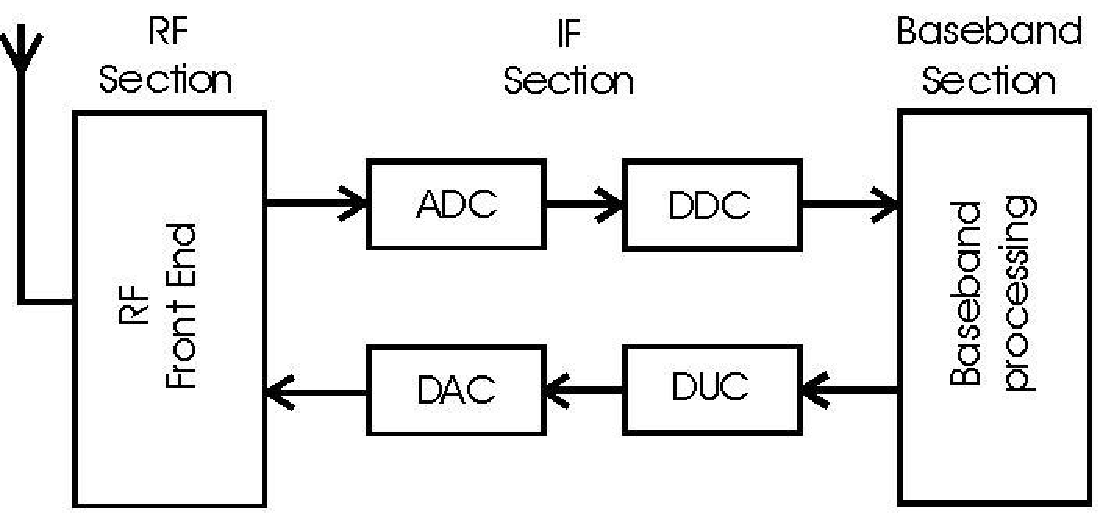
\includegraphics[width=0.7\textwidth]{../images/sdrBlock}
  \caption{Block diagram of SDR.}
  \label{sdrBlock}
\end{figure}

The \gls{sdr} contains a number of basic functional blocks.
The \gls{sdr} in general can be divided into three basic sections, namely the front
end, the IF section and the base-band section. The front end section consits 
of analogue RF circuitry that is responsible for the reception and 
transmission of signals at the operating frequency. The IF section performs
the digital to analog conversion and vice versa. It also does various signal 
processing tasks like filtering, modulation and demodulation, digital up 
conversion (DUC), digital down conversion (DDC) etc. The last stage of the 
radio is the baseband processor. This is the point where the digital data 
gets processed \cite{miller08}\cite{kranthi13}.
We have used GNURadio and \gls{usrp} N210 to configure the \gls{sdr} used in implementing
our Cognitive Radio Test-Bed. 

\begin{figure}
  \centering
  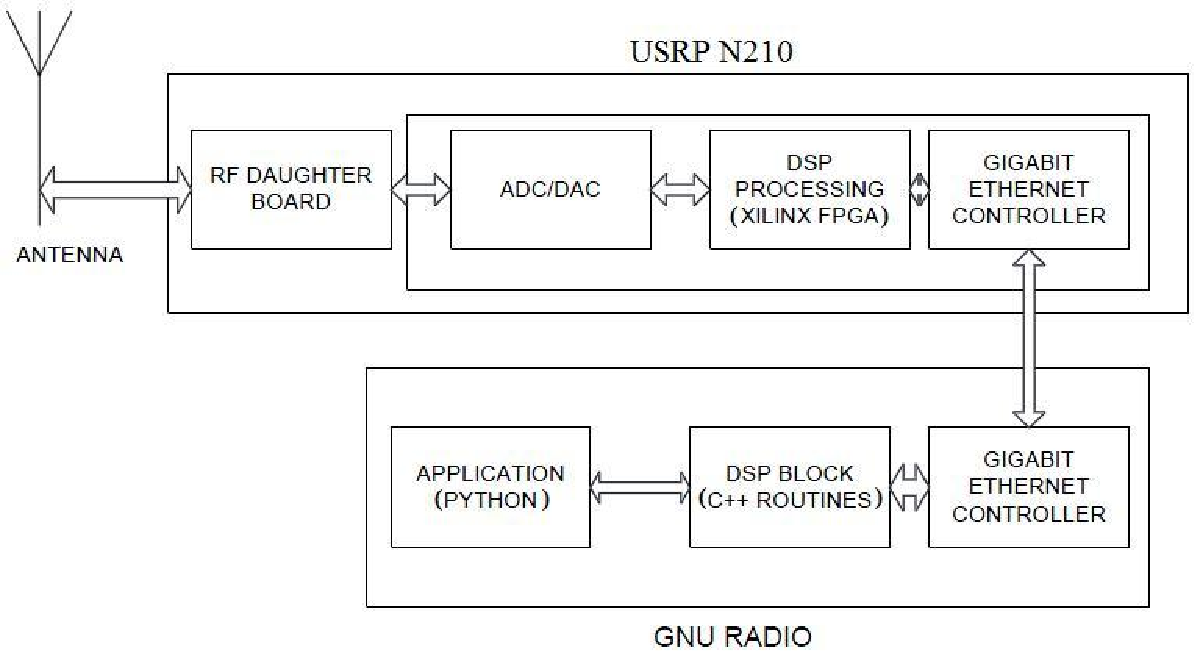
\includegraphics[width=0.7\textwidth]{../images/usrpGNURadioBlock}
  \caption[USRP operation with GNURadio]{Block diagram for the operation of USRP
  with GNURadio.}
  \label{usrpGNURadioBlock}
\end{figure}

A block diagram of a \gls{usrp}-based \gls{sdr} transceiver executing a GNURadio based 
application is shown in Figure \ref{usrpGNURadioBlock}. The \gls{usrp} kit is the 
hardware interface and GNURadio is used for the baseband signal processing
tasks.


\section{\gls{usrp}}

The \gls{usrp} is intended to provide a 
low-cost, high quality hardware platform for software radio. It is designed
and marketed by Ettus Research, LLC. It is commonly used by research labs,
universities, and hobbyists. The \gls{usrp} platform is designed for RF applications
from DC to 6 GHz. \gls{usrp}s connect to a host computer through a high-speed USB or
Gigabit Ethernet link, which the host-based software uses to control the \gls{usrp}
hardware and transmit/receive data.

The \gls{uhd} is the official driver for all Ettus Research
products. The \gls{uhd}supports Linux, Mac OS X and Windows.

\begin{figure}
\centering
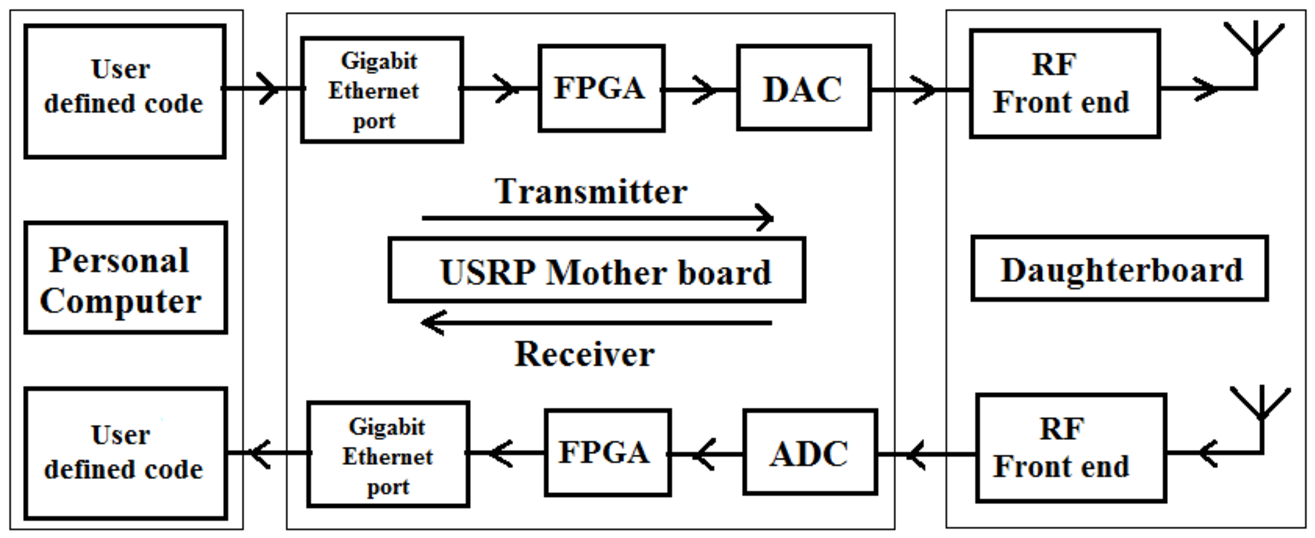
\includegraphics[width=0.9\textwidth]{../images/usrpBlock}
\caption[Block diagram of USRP]{Block diagram of USRP
\protect\cite{kranthi13}.}
\label{usrpBlock}
\end{figure}

In this project we are using a particular model of the \gls{usrp} known as the
\gls{usrp} N210.

\subsection{\gls{usrp} N210}

The \gls{usrp} N200 and N210 are the highest performing class of hardware of the 
\gls{usrp} family of products, which enables engineers to rapidly design and 
implement powerful, flexible software radio systems. The N200 and N210 
hardware is ideally suited for applications requiring high RF performance and
great bandwidth. Such applications include physical layer prototyping, dynamic
spectrum access and cognitive radio, spectrum monitoring, record and playback,
and even networked sensor deployment. The Networked Series products offers 
MIMO capability with high bandwidth and dynamic range. The Gigabit Ethernet
interface serves as the connection between the N200/N210 and the host 
computer. This enables the user to realize 50 MS/s of real-time bandwidth in 
the receive and transmit directions, simultaneously (full duplex).


\section{GNURadio}

GNURadio is a free \& open-source software development toolkit that provides 
signal processing blocks to implement software radios. It can be used with 
readily-available low-cost external RF hardware to create software-defined 
radios, or without hardware in a simulation-like environment. It is widely 
used in hobbyist, academic and commercial environments to support both 
wireless communications research and real-world radio systems.

\subsection{What does GNURadio do?}
It does all the signal processing. It can be used to write applications to 
receive data out of digital streams or to push data into digital streams, 
which is then transmitted using hardware.

GNURadio has software equivalents of real world radio system components like 
filters, demodulators, equalizers, etc. These are usually referred to as
blocks. You can create a complex system by connecting various blocks. If you
cannot find some specific blocks, you can even create your own blocks and add
them.

Most of GNURadio has been implemented using the Python programming language,
and the performance-critical parts have been implemented using C++. Typically,
a GNURadio user writes his applications in Python, unless he has some
performance-critical needs. Thus, GNURadio gives its users an easy-to-use,
rapid application development environment.

\subsection{GNURadio with \gls{usrp}}

\begin{figure}
\centering
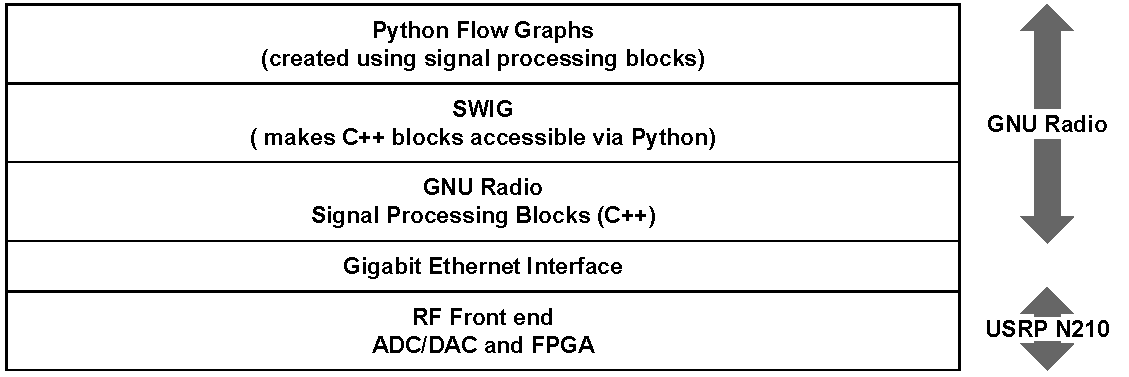
\includegraphics[width=0.9\textwidth]{../images/gnuradio_architecture}
\caption{Architecture of GNURadio}
\label{gnuradio_architecture}
\end{figure}

The \gls{usrp} and the host computer make up the hardware part of the \gls{sdr} system. 
The host computer must run a compatible software package such as GNURadio or
Simulink to complete the \gls{sdr} system. In this project we are using GNURadio
as the software platform.

GNURadio communicates with the \gls{usrp} through the \gls{uhd}
software. The \gls{uhd}provides a host driver and an Application Programming
Interface (API) for the \gls{usrp}. GNURadio uses the \gls{uhd}to set user-specified
parameters like RF center frequency, antenna selection, gain, sampling rate,
interpolation, decimation, etc.

